% Filter Circuits with Bode Plots
% Demonstrates: RC low-pass, RL high-pass, RLC bandpass with frequency response.
% Compile with: pdflatex main.tex

\documentclass{article}
\usepackage[american, siunitx]{circuitikz}
\usepackage{pgfplots}
\pgfplotsset{compat=1.18}
\usepackage{amsmath}

\title{Filter Circuits and Bode Plots}
\author{LaTeX Tutorial}
\date{\today}

\begin{document}
\maketitle

% =============================================================================
\section{RC Low-Pass Filter}
% =============================================================================

\begin{center}
\begin{circuitikz}[scale=1]
    \draw (0,0) to[R, l=$R$, o-] (3,0)
        to[C, l=$C$] (3,-2)
        -- (0,-2) to[open, o-] (0,0);
    \draw (3,0) to[short, -o] (5,0);
    \draw (3,-2) to[short, -o] (5,-2);
    \node[left] at (0, -1) {$V_{\text{in}}$};
    \node[right] at (5, -1) {$V_{\text{out}}$};
\end{circuitikz}
\end{center}

Transfer function: $H(j\omega) = \dfrac{1}{1 + j\omega RC}$, \quad
cutoff: $f_c = \dfrac{1}{2\pi RC}$

\begin{center}
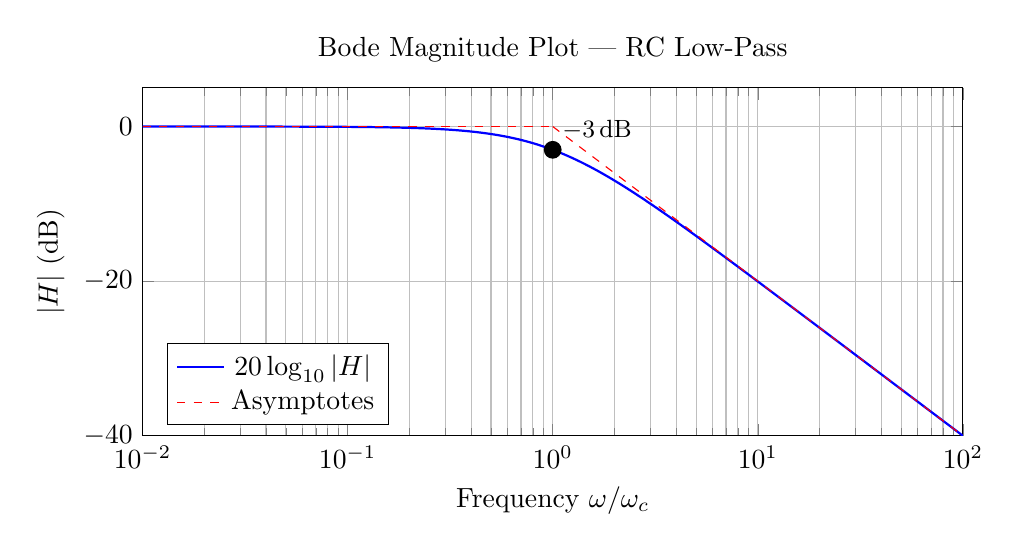
\begin{tikzpicture}
\begin{semilogxaxis}[
    width=12cm, height=6cm,
    title={Bode Magnitude Plot --- RC Low-Pass},
    xlabel={Frequency $\omega / \omega_c$},
    ylabel={$|H|$ (dB)},
    xmin=0.01, xmax=100,
    ymin=-40, ymax=5,
    grid=both,
    legend pos=south west,
]
    \addplot[thick, blue, domain=0.01:100, samples=200]
        {-10*log10(1 + x^2)};
    \addlegendentry{$20\log_{10}|H|$}

    % Asymptotes
    \addplot[dashed, red, domain=0.01:1] {0};
    \addplot[dashed, red, domain=1:100] {-20*log10(x)};
    \addlegendentry{Asymptotes}

    % -3dB point
    \addplot[only marks, mark=*, mark size=3pt, black]
        coordinates {(1, -3.01)};
    \node[above right, font=\small] at (axis cs:1,-3) {$-3$\,dB};
\end{semilogxaxis}
\end{tikzpicture}
\end{center}

% =============================================================================
\section{RL High-Pass Filter}
% =============================================================================

\begin{center}
\begin{circuitikz}[scale=1]
    \draw (0,0) to[C, l=$C$, o-] (3,0)
        to[R, l=$R$] (3,-2)
        -- (0,-2) to[open, o-] (0,0);
    \draw (3,0) to[short, -o] (5,0);
    \draw (3,-2) to[short, -o] (5,-2);
    \node[left] at (0, -1) {$V_{\text{in}}$};
    \node[right] at (5, -1) {$V_{\text{out}}$};
\end{circuitikz}
\end{center}

Transfer function: $H(j\omega) = \dfrac{j\omega RC}{1 + j\omega RC}$

\begin{center}
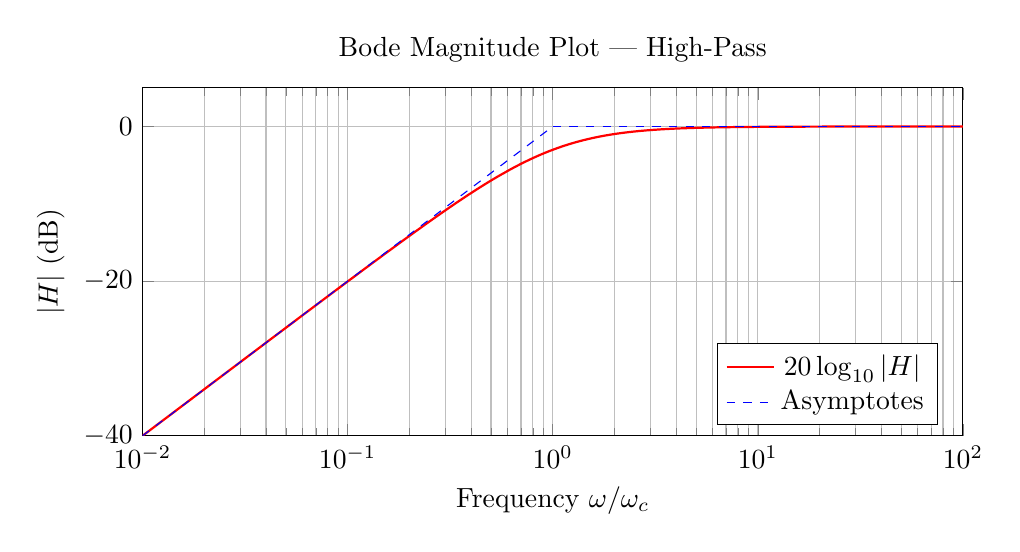
\begin{tikzpicture}
\begin{semilogxaxis}[
    width=12cm, height=6cm,
    title={Bode Magnitude Plot --- High-Pass},
    xlabel={Frequency $\omega / \omega_c$},
    ylabel={$|H|$ (dB)},
    xmin=0.01, xmax=100,
    ymin=-40, ymax=5,
    grid=both,
    legend pos=south east,
]
    \addplot[thick, red, domain=0.01:100, samples=200]
        {-10*log10(1 + 1/x^2)};
    \addlegendentry{$20\log_{10}|H|$}

    % Asymptotes
    \addplot[dashed, blue, domain=0.01:1] {20*log10(x)};
    \addplot[dashed, blue, domain=1:100] {0};
    \addlegendentry{Asymptotes}
\end{semilogxaxis}
\end{tikzpicture}
\end{center}

% =============================================================================
\section{RLC Bandpass Filter}
% =============================================================================

\begin{center}
\begin{circuitikz}[scale=1]
    \draw (0,0) to[L, l=$L$, o-] (2,0)
        to[C, l=$C$] (4,0)
        to[short] (4,0);
    \draw (4,0) to[R, l=$R$] (4,-2)
        -- (0,-2) to[open, o-] (0,0);
    \draw (4,0) to[short, -o] (6,0);
    \draw (4,-2) to[short, -o] (6,-2);
    \node[left] at (0, -1) {$V_{\text{in}}$};
    \node[right] at (6, -1) {$V_{\text{out}}$};
\end{circuitikz}
\end{center}

Resonant frequency: $f_0 = \dfrac{1}{2\pi\sqrt{LC}}$, \quad
Quality factor: $Q = \dfrac{1}{R}\sqrt{\dfrac{L}{C}}$

\begin{center}
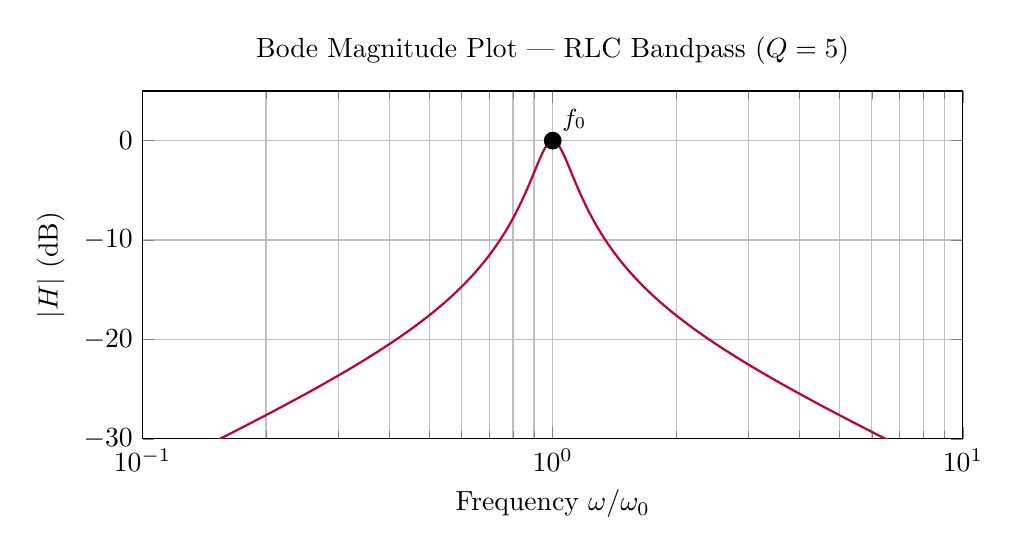
\begin{tikzpicture}
\begin{semilogxaxis}[
    width=12cm, height=6cm,
    title={Bode Magnitude Plot --- RLC Bandpass ($Q=5$)},
    xlabel={Frequency $\omega / \omega_0$},
    ylabel={$|H|$ (dB)},
    xmin=0.1, xmax=10,
    ymin=-30, ymax=5,
    grid=both,
]
    % Q=5 bandpass: H = jw/(Q) / (1 - w^2 + jw/Q), |H|^2 = (w/Q)^2/((1-w^2)^2+(w/Q)^2)
    \addplot[thick, purple, domain=0.1:10, samples=300]
        {10*log10( (x/5)^2 / ((1-x^2)^2 + (x/5)^2) )};

    % Resonance marker
    \addplot[only marks, mark=*, mark size=3pt, black]
        coordinates {(1, 0)};
    \node[above right, font=\small] at (axis cs:1,0) {$f_0$};
\end{semilogxaxis}
\end{tikzpicture}
\end{center}

\end{document}
